\documentclass[10pt,a4paper]{amsart}
\usepackage[margin=19mm]{geometry}
\usepackage{amsmath,amssymb,mathtools}
\usepackage[scr=rsfs,cal=euler]{mathalfa}
\usepackage{xfrac}
\usepackage[unicode,hidelinks,bookmarks=false]{hyperref}
\newcommand{\ie}{i.e.\ }
\newcommand{\cf}{cf.\ }
\newcommand{\resp}{respectively\ }
\newcommand{\Subsection}{\subsection}
\providecommand{\nobreakdash}{\nobreak\hbox{-}}
\setlength{\emergencystretch}{2em}
\multlinegap0pt
\usepackage{tikz}
\usepackage{enumerate}
\usepackage{amssymb}
\usepackage{xcolor}
\usepackage{float}
\newtheorem{lem}{Lemma}
\newtheorem{rem}{Remark}
\newtheorem{scope}{Scope}
\title{Chebyshev's method applied to polynomials with rotational symmetry}
\author{Tarakanta Nayak, Pooja Phogat}
\date{Source: arXiv:2609.02884v1 (CC BY 4.0)}
\begin{document}
\maketitle

\noindent\emph{Source and licence.} Chebyshev's method applied to polynomials with rotational symmetry. Version arXiv:2609.02884v1 (CC BY 4.0), distributed by arXiv under the Creative Commons Attribution 4.0 International licence, http://creativecommons.org/licenses/by/4.0/, as recorded in the arXiv licence metadata for this exact version and shown on the abstract page https://arxiv.org/abs/2609.02884v1. Full licence notice: \texttt{licenses/arxiv-2609.02884-CC-BY-4.0.txt}.\par\smallskip

\noindent\textit{Editorial scope.} Counted unit: the article's lem Non-A\_1 (source0.tex lines 873--875). The article's complete original proof of it is delivered with it (source0.tex lines 877--957, one \texttt{proof} environment of 81 lines). No mathematics is written, repaired or re-derived: the statement and the proof are the article's own lines, in the article's own notation, and no retained line is substituted or re-flowed.  Retained uncounted as the source-local context the proof needs: lines 721--735; lines 758--762.  Nothing was omitted from any retained span, so the package carries no omission record.  No retained line contains a citation, so the wrapper carries no bibliography and no bibliography entry.  The retained lines contain the article's own diagram code, which the wrapper typesets with the standard tikz packages; no image file is delivered and the package declares no asset dependency.  Editorial formatting only, in addition: an AMS \texttt{amsart} preamble that restates the article's own declarations and macros used by the retained lines, namely the environments \texttt{lem}, \texttt{rem}, \texttt{scope} on separate counters, together with the standard packages those lines need.  The retained environments print in this document as Lemma 1, Remark 1, Scope 1 in order of appearance, whereas the article prints the same items with the numbering of its own full document.  The complete native source of the article as distributed in the arXiv e-print for this exact version is bundled unchanged as \texttt{sources/209250/source0.tex}.
\begin{lem}(Symmetry about  lines) \label{Inv_lines_ref-sym}
	For each $k \in \{ 0, 1, \dots, n-1\}$, let $\lambda_{k} = \exp\left(\frac{k\pi i}{n}\right)$ and  $L_{k} = \left\{ \lambda_k t : t \in \mathbb{R}\right\}$. Then the following statements hold.
	\begin{enumerate}
		\item The map $C_{n}$ satisfies $C_n (z)=\lambda_k ^{-2} \overline{(C_n (\lambda_k ^2 \overline{z}))}$, i.e., $C_n$ is symmetric with respect to the line $L_k$ for each $k$. In particular, each line $L_k$ is invariant under $C_{n}$. 
		\item If  $k$ is odd, then 
	$C_{n}(\lambda_{k} z) = \lambda_{k} Q_n (z)$ for all $z,$  where 
	\begin{equation}
		Q_n(z)= \frac{z^{n+1} \big(n(n+1)(2n+1)z^{2n} + 2n(n+1)z^{n} - n(n-1)\big)}{2\big((n+1)z^{n} + 1\big)^3}.
		\label{Q_conj} 
	\end{equation} 
		\item 	If $k$ is even, then 
		$C_{n}(\lambda_{k} z) = \lambda_{k} C_{n}(z)$ for all $z.$ 
	
	\end{enumerate}  
\end{lem}

\begin{rem}
	For $k=0$, Lemma~\ref{Inv_lines_ref-sym}(1) gives that 
	$C_n (z)=\overline{C_n(\overline{z})}$, i.e., $C_n$ is symmetric about the real line.
	\label{symm-R}
\end{rem}

	\begin{lem}\label{Non-A_1}
	The immediate basin	$\mathcal{A}_1$ cannot contain any negative real number.
	\end{lem}	

	\begin{proof}
		Suppose, on the contrary, that $\mathcal{A}_1$ contains a negative real number, say $a^{-}$. Since $\mathcal{A}_1$ is connected, there exists a simple arc $\gamma$ in $\mathbb{C} \cap \mathcal{A}_1$ joining $1$ and $a^{-}$. Because the origin belongs to  $\mathcal{A}_0$ and $\mathcal{A}_1 \cap \mathcal{A}_0 = \emptyset$, the arc $\gamma$ cannot lie entirely on the real line. Moreover, since $\mathcal{A}_1$ is symmetric with respect to the real line (a consequence of Remark~\ref{symm-R}), the reflected arc $\bar{\gamma} := \{\overline{z}: z\in \gamma\}$ is also contained in $\mathcal{A}_1$. It follows that $\Gamma = \gamma \cup \bar{\gamma}$ forms a closed curve enclosing the origin. Since $\mathcal{A}_2 = \sigma(\mathcal{A}_1)$, where $\sigma(z) = e^{\frac{2\pi  i}{n}}z$, the rotated curve $\sigma(\Gamma)$ lies entirely in $\mathcal{A}_2$ and also encloses the origin. Therefore $\Gamma \cap \sigma(\Gamma) \neq \emptyset$, which implies that $\mathcal{A}_1 \cap \mathcal{A}_2 \neq \emptyset$ (see Figure~\ref{loops_Intersect}). This is a  contradiction,  thereby completing the proof.
	%%%%%%%%%%%%%%%%%%%%%%%%%%%%%%%
	\begin{figure}[htbp]
		\centering
		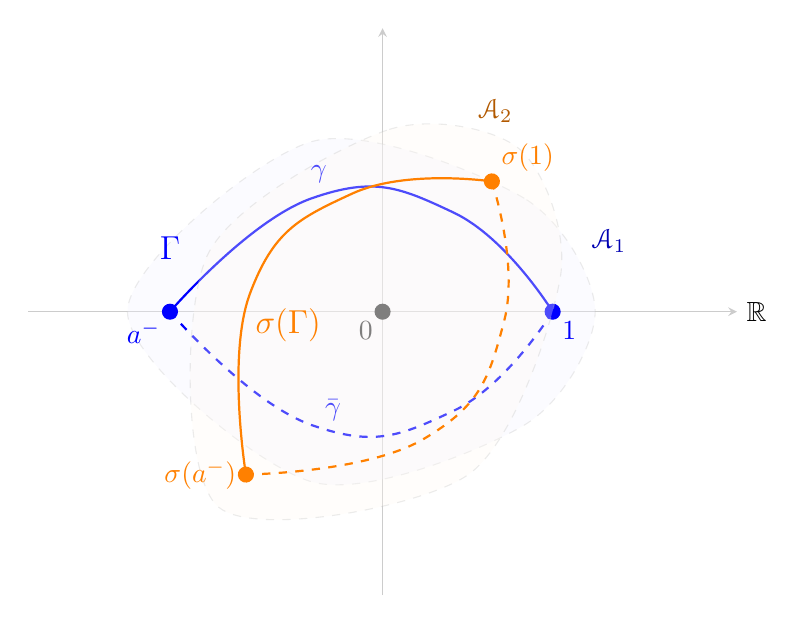
\begin{tikzpicture}[scale=1.8, >=stealth]
			
			% Grid/Axis lines for reference (faint grey)
			\draw[->, help lines, color=gray!40, thin] (-2.5,0) -- (2.5,0) node[right, black] {$\mathbb{R}$};
			\draw[->, help lines, color=gray!40, thin] (0,-2) -- (0,2);
			
			% Origin point
			\filldraw[black] (0,0) circle (1.5pt) node[below left] {$0$};
			
			% --- SECTION 1: A_1 and \Gamma ---
			% Domain A_1 boundary (Light blue, symmetric background hint)
			\draw[lightgray, dashed, fill=blue!5, opacity=0.3] plot[smooth cycle] coordinates {
				(1.5,0) (1,0.8) (-0.5,1.2) (-1.8,0) (-0.5,-1.2) (1,-0.8)
			};
			\node[blue!70!black] at (1.6, 0.5) {$\mathcal{A}_1$};
			
			% Point 1 and a^-
			\filldraw[blue] (1.2, 0) circle (1.5pt) node[below right] {$1$};
			\filldraw[blue] (-1.5, 0) circle (1.5pt) node[below left] {$a^-$};
			
			% Upper arc \gamma (passing above the origin)
			\draw[thick, blue] plot[smooth, tension=0.8] coordinates {
				(1.2,0) (0.5,0.7) (-0.5,0.8) (-1.5,0)
			};
			\node[blue, above] at (-0.45, 0.84) {$\gamma$};
			
			% Lower arc \bar{\gamma} (symmetric reflection)
			\draw[thick, blue, dashed] plot[smooth, tension=0.8] coordinates {
				(1.2,0) (0.5,-0.7) (-0.5,-0.8) (-1.5,0)
			};
			\node[blue, below] at (-0.35, -0.55) {$\bar{\gamma}$};
			
			% Label for \Gamma
			\node[blue, font=\large] at (-1.5, 0.45) {$\Gamma$};
			
			
			% --- SECTION 2: A_2 and \sigma(\Gamma) ---
			% Rotation angle line for visual aid (e^{i\pi/n} where n is roughly 3 or 4 here)
			% Let's rotate by 50 degrees
			\begin{scope}[rotate=50]
				% Domain A_2 boundary hint
				\draw[lightgray, dashed, fill=orange!5, opacity=0.3] plot[smooth cycle] coordinates {
					(1.5,0) (1,0.8) (-0.5,1.2) (-1.8,0) (-0.5,-1.2) (1,-0.8)
				};
				\node[orange!70!black] at (1.6, 0.3) {$\mathcal{A}_2$};
				
				% Rotated upper arc
				\draw[thick, orange] plot[smooth, tension=0.8] coordinates {
					(1.2,0) (0.5,0.7) (-0.5,0.8) (-1.5,0)
				};
				
				% Rotated lower arc
				\draw[thick, orange, dashed] plot[smooth, tension=0.8] coordinates {
					(1.2,0) (0.5,-0.7) (-0.5,-0.8) (-1.5,0)
				};
				
				% NEW: Orange dots at the endpoints inside the rotated scope
				\filldraw[orange] (1.2, 0) circle (1.5pt) node[above right] {$\sigma(1)$};
				\filldraw[orange] (-1.5, 0) circle (1.5pt) node[left] {$\sigma(a^-)$};
				
				% Label for \sigma(\Gamma)
				\node[orange, font=\large] at (-0.5, 0.45) {$\sigma(\Gamma)$};
			\end{scope}
			
			% % --- INTERSECTION HIGHLIGHT ---
			% Mark one of the clean intersection points where the loops cross to emphasize \Gamma \cap %\sigma(\Gamma) \neq \emptyset
			% \filldraw[red] (-0.32, 0.68) circle (1.8pt);
			% \filldraw[red] (0.32, -0.68) circle (1.8pt);
			% \draw[red, <-] (-0.28, 0.72) .. controls (-0.1, 1.2) and (0.3, 1.2) .. (0.6, 1.3)
			% node[right, black, font=\small] {Intersection $\Gamma \cap \sigma(\Gamma) \neq \emptyset$};
			
		\end{tikzpicture}
		\caption{Illustration of the contradiction arising from the intersection of $\Gamma$ and $\sigma(\Gamma)$.}
		\label{loops_Intersect}
	\end{figure}
\end{proof}	

\end{document}
